\documentclass[a4paper, 12pt]{article}
\usepackage{geometry}
\geometry{a4paper,
total={170mm,257mm},left=2cm,right=2cm,
top=2cm,bottom=2cm}

\usepackage{mathtext}
\usepackage{amsmath}
\usepackage[T2A]{fontenc}
\usepackage[utf8]{inputenc}
\usepackage[english,russian]{babel}
\usepackage{graphicx, float}
\usepackage{tabularx, colortbl}
\usepackage{caption}
\captionsetup{labelsep=period}

\newcommand{\parag}[1]{\paragraph*{#1:}}
\DeclareSymbolFont{T2Aletters}{T2A}{cmr}{m}{it}
\newcounter{Points}
\setcounter{Points}{1}
\newcommand{\point}{\arabic{Points}. \addtocounter{Points}{1}}
\newcolumntype{C}{>{\centering\arraybackslash}X}

\author{Калинин Даниил, Б01-110}
\date{\today}
\title{Лабораторная работа 2.2.5\\Определение вязкости жидкости по скорости истечения из капилляра}

\begin{document}
\maketitle

\parag {Цель работы}
\begin{enumerate}
    \item определенить вязкость воды по измерению объёма жидкости, протёкшей через капилляр.
\end{enumerate}

\parag {В работе используются}
\begin{itemize}
    \item сосуд Мариотта
    \item капиллярная трубка
    \item мензурка
    \item секундомер
    \item микроскоп на стойке
\end{itemize}

\parag {Теоритическая справка} ~\\
Используя формулу Пуазейля:
    \begin{equation}
        Q = \pi \frac{P_1-P_2}{8 \eta l} R^4
        \label{eq:Puaz}
    \end{equation}

Мы можем расчитать вязкость жидкости, зная расход жидкости $Q$, радиус трубки токи $R$, длину трубки $l$ и перепад давлений $P_1 - P_2$ на концах трубки тока. 

Для нас важно, чтобы поток жидкости внутри капилляра был ламинарным, а разность давлений постоянной. 

Характер течения газа или жидкости зависит от соотношения между кинетической зпергией движущейся среды и работой сил вязкости. Если первая величина мала по сравнению со второй, то турбулентные пульсации пе развиваются, их подавляет вязкость и течение остается ламиарным. Отношение кинетической энергии некоторого объема таза или жидкости $\rho v^2 L$ к работе вязких сил на характерной длине $\eta (\frac{v}{L}) L^2$ определяет безразмерное число Рейнольдса:
\begin{equation}
    Re = \frac{v R \rho}{\eta} = \frac{2 \frac{\rho v^2}{2}}{\eta \frac{v}{R}} = \frac{QR \rho}{S \eta} = \frac{V\rho}{\pi R \eta t}
    \label{eq:Rayan}
\end{equation}

В гладких трубах круглого сечения переход от ламинарного движения к турбулентному происходит при $Rе \approx 1000$.

Прежде чем применять формулу Пуазейля к конкретным расчетам, всегда следует убедиться в том, что течение жидкости является ламинарным. Ламинарное движение жидкости при переходе ее из широкого сосуда в капилляр устанавливается не сразу, а после того, как она пройдет расстояние $a$:
\begin{equation}
    a = 0.2R - Re
    \label{eq:A}
\end{equation}

Формула \ref{eq:Puaz} дает надежные результаты лишь в том случае, вели длина капилляра во много раз больше $a$.

\parag {Экспериментальная установка}~\\
Установка для измерения вязкости воды изображена на рис. \ref{fig:vac}. 

\begin{figure}[h]
    \centering
    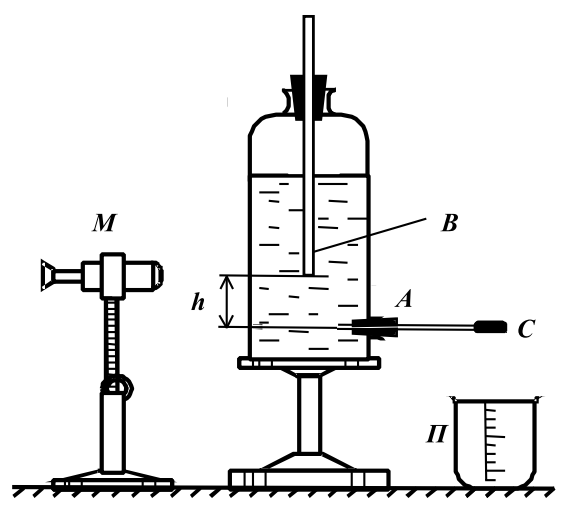
\includegraphics[width=7cm]{setup1.PNG}
    \caption{Схема установки для определения вязкости воды}
    \label{fig:vac}
\end{figure}

Вода заполняет сосуд Мариотта и вытекает через калиброванную капиллярную трубку, укрепленную в нижней части его боковой стенки. Сосуд Мариотта позволяет поддерживать постоянным перепад давления $P_1 - P_2$ на концах капилляра, несмотря на то, что уровень жидкости при ее вытекании понижается. Это достигается с помощью трубки $В$, открытой в атмосферу и проходящей через пробку, герметично закрывающую сосуд.

Величина перепада давления $P_1 - P_2$ определяется высотой столба воды $h$ между осью капиллярной трубки $А$ и нижним концом вертикальной трубки $В$. Высота столба измеряется с помощью микроскопа $М$, укрепленного на вертикально перемещающемся плунжере. Смещение плунжера определяется по миллиметровой шкале, снабженной нониусом. Объем вытекшей жидкости измеряется мензуркой $П$. Время истечения определяется по секундомеру. Длина капиллярной трубки измеряется миллиметровой линейкой, диаметр -- микроскопом МИР.

\parag {Ход работы} ~\\

\point С помощь микроскопа определим радиус трубки: $R = 0,4 \pm 0.05$ мм.

\point С помощью миллиметровой линейки определим длину капилляра: $l = 137 \pm 0.5$ мм.

\point Убедимся, что расход воды при одинаковой величине $h$ не зависит от уровня жидкости. При $h = 30.7$ мм. объём 20 см$^3$ вытек из сосуда сначала за 709 с, затем за 701 с. Таким образом, условие выполняется.

\point Перепад давлений $\Delta P = P_1 - P_2$ на концах капилляра, выраженный в миллиметрах водяного столба, не равен $h$, а содержит поправку $\Delta h$, обусловленную силами поверхностного натяжения. Чтобы её определить, будем опускть трубку $В$ до тех пор, пока вода не перестанет вытекать из капилляра. Наступление этого момента значит, что давление столба воды $\Delta h$ между осью капилляра и нижним торцом трубки $В$ уравновесилось силами поверхностного натяжения пузырька воздуха, возникшего на конце трубки $В$, и капли жидкости на конце капилляра.

Таким образом, получим:
\begin{equation*}
    \Delta h = 1.17~cм.
\end{equation*}

Тогда разность давлений $P_1 - P_2$, можно расчитать так:
\begin{equation}
    \Delta P = P_1 - P_2 = (h - \Delta h)\rho g
    \label{deltaP}
\end{equation}

\point Измерим расход воды при нескольких значениях $h$. По формуле \ref{eq:Rayan} для числа Рейнольдса удостоверимся, что в каждом из опытов в капилляре устанавливается ламинарное течение. По формуле \ref{eq:A} оценим длину участка капилляра, по прохождении которого устанавливается ламинарное течение.  Результаты занесём в таблицу \ref{tabl:data}. 

\begin{table}[h]
    \centering
    \begin{tabular}{|c|c|c|c|c|c|}
    \hline 
    $h$, см.&   $t$, с. &   $V$, см$^3$.& $Q$, см$^3$/с.&   $Re$    &   $a$, см.    \\ \hline
    3.07	&	709	    &	20	        &	0.0282	    &	22.448	&	0.180	    \\
    3.41	&	434	    &	20	        &	0.0461	    &	36.672	&	0.293	    \\
    4.0	    &	315	    &	20	        &	0.0635	    &	50.525	&	0.404	    \\
    4.73	&	275	    &	20	        &	0.0727	    &	57.875	&	0.463	    \\
    5.12	&	222	    &	20	        &	0.0901	    &	71.691	&	0.574	    \\
    7.05	&	164	    &	20	        &	0.1220	    &	97.046	&	0.7 76	    \\ \hline
    \end{tabular}
	\caption{Результаты экспериментов}
    \label{tabl:data}
\end{table}

\point Полученную зависимость $Q(h)$ изобразим на графике (рис. \ref {pic:graph}). 

\begin{figure}[h]
    \centering
    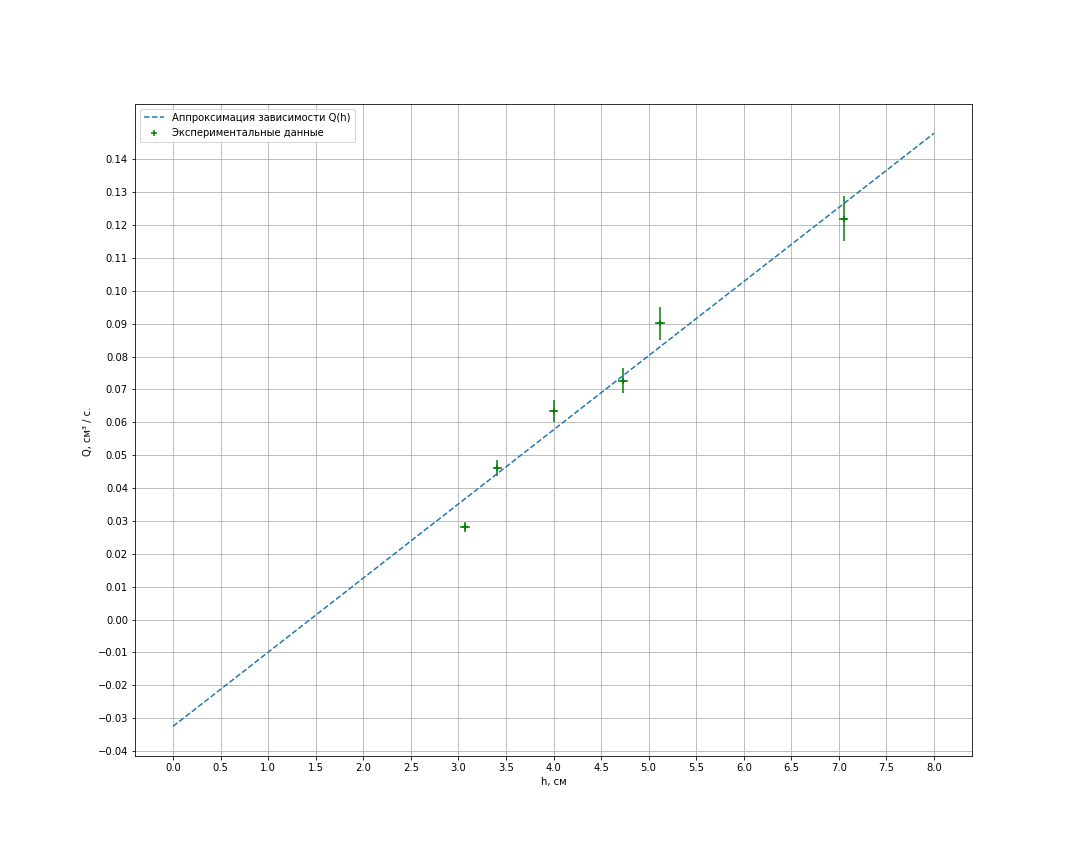
\includegraphics[width=\linewidth]{graph.png}
    \caption{Зависимость расхода $Q$ от расстояния между осью капилляра и трубкой $h$.}
    \label{pic:graph}
\end{figure}

\point Из графика можно определить расчитанное ранее расстояние $\Delta h$. Оно будет равно пересечению нашей прямой и прямой $Q = 0$. Зная параметры прямой, получаем:
\begin{equation*}
    \Delta h_{Экспериментальное} = 1.44~cм.
\end{equation*}
Как видно, полученное значение хорошо согласуется с расчитанным.

\point Воспользовавшись формулой Пуазейля (\ref{eq:Puaz}) и формулой для разности давлений (\ref{deltaP}), выведем формулу для расчета $\eta$ (\ref{eq:eta_formula}).

\begin{equation}
    \eta = \frac{\pi R^4 \rho g}{8 l Q'(h)}
    \label{eq:eta_formula}
\end{equation}

Подставив в формулу \ref{eq:eta_formula} коэффициент наклона прямой на графике, получим:

\begin{equation*}
    \eta = 0.00779~П
\end{equation*}

Оценим погрешность определения вязкости по формуле
\begin{equation*}
    \sigma \eta = \eta \sqrt{(\frac{\sigma h}{h})^2 + 4^2(\frac{\sigma R}{R})^2 + (\frac{\sigma l}{l})^2} = 0.000328~П
\end{equation*}
    
Для воды температуры 25$^{\circ} $C значение вязкости $\eta = 0.00891$ П. \par

С учётом погрешности, определенная нами вязкость сходится с табличным значением.

Таким образом:
\begin{equation*}
    \eta_{water} = 0.00778 \pm 0.000328
\end{equation*}


\parag {Заключение} ~\\
В ходе работы былa определена вязкость воды по измерению объёма жидкости, прошедшей через капилляр. Значение вязкости воды, полученное экспериментальным способом, совпадает с табличным практически полностью.
\end{document}
